\chapter{Interacción Débil}\label{cap:weak_int}
El origen de cada interacción fundamental se debe a causas diferentes. Por un lado, la existencia de carga eléctrica produce fuerzas electromagnéticas en las partículas y las hace interactuar entre sí, mientras que la interacción fuerte se debe a la propiedad del color, mencionada en el capítulo anterior. No todas las partículas tienen carga ni color simultáneamente por lo que no todas son susceptibles a las mismas interacciones. El caso de la interacción débil es bastante interesante porque muchas partículas con propiedades distintas son sensibles a ella. Por ejemplo, los leptones no tienen carga de color, no ``sienten'' la interacción fuerte; pero los neutrinos no tienen carga eléctrica por lo que no pueden interactuar mediante fuerzas electromagnéticas. Sin embargo, ambos tipos de partículas pueden estar presentes en interacciones débiles.\cite{Griffiths2008} Además, la causa de la interacción débil, aunque no tiene un nombre específico, comúnmente se denota como \textit{carga débil}.

Los mesones $K$ y muchas otras partículas decaen por interacción débil. Desde el principio se consideró un tratamiento cuántico-relativista para su descripción y muchos científicos han contribuido al desarrollo de su formalismo. Cada interacción ocurre gracias al intercambio de una partícula mediadora o portadora de la fuerza de interacción. En la interacción fuerte es el gluón y en la electromagnética es el fotón. Sin embargo, en lo que respecta a la interacción débil, esas partículas mediadoras encargadas de transmitir la fuerza débil entre los quarks y leptones, son los bosones vectoriales, llamados así porque tienen espín 1. Debido a su gran masa, se tiene en consecuencia que la interacción débil es de muy corto alcance. Estos bosones portadores de la fuerza débil pueden ser cargados $W^{\pm}$ o neutros $Z^0$, dependiendo de las partículas que participan en el proceso. 

Hasta la década de los 70, sólo se habían observado procesos de intercambio de bosones cargados $W^{\pm}$. En los años 60 se empezó a formular una teoría que aunaba la interacción débil junto con la electromagnética, en lo que se conoce hoy en día como \textit{Teoría Electrodébil}. Esta teoría predecía la existencia del bosón neutro mediador de la fuerza débil y dicha hipótesis fue confirmada experimentalmente en 1973 \cite{BrianM}, con el descubrimiento de $Z^0$.

Este capítulo se centra, principalmente, en la descripción de procesos de interacción débil cargados con intercambio de bosones $W^{\pm}$ y nos servirá como base para el estudio del decaimiento de mesones $K$ cargados.

\section{Formalismo de la Interacción Débil}\label{cap:formalism}
\subsection{Interacciones en Teoría Cuántica de Campos}\label{sec:qft}
De acuerdo con la Teoría Cuántica de Campos (TCC), cada partícula lleva asociado un campo cuántico $\phi(x)$, $\psi(x)$ o $W_{\mu}(x)$, dependiente del espacio y del tiempo $x^{\mu}=(ct,\boldsymbol{\vec{x}})$\protect\footnotemark. Estos campos $\phi(x)$, $\psi(x)$ o $W_{\mu}(x)$ actúan como operadores encargados de aniquilar partículas o crear antipartículas de espín $0$, $1/2 $ y $1$, respectivamente \cite{notas2020}.

\footnotetext{Consultar el Apéndice \hyperref[cap:A]{A} para más información sobre la notación utilizada en este capítulo.}
 
Para describir la evolución espacio-temporal de dichos campos asociados a partículas se hace uso de la densidad lagrangiana $\mathcal{L}$. Para las distintas partículas y sin tener en cuenta la interacción, en el sistema natural de unidades ($c=\hbar =1$), $\mathcal{L}$ tiene las siguientes expresiones:
\begin{itemize}
\item Bosones de espín $0$, tales como los mesones $K$ o los piones:
\end{itemize}
\begin{equation*}
\mathcal{L}=-\partial ^{\mu }\phi \left( x\right) ^{\ast }\partial_{\mu} \phi \left( x\right) -m^{2}\phi \left( x\right) ^{\ast }\phi \left( x\right)
\end{equation*}
El campo $\phi(x)$ tiene carácter escalar y es responsable de (crear) aniquilar (anti)partículas con $J=0$. $\phi^{\ast}(x)$ es su campo conjugado y hace justo lo opuesto: crea partículas y aniquila antipartículas con $J=0$.
\begin{itemize}
\item Fermiones de espín $1/2$, como los leptones:
\end{itemize}
\begin{equation*}
\mathcal{L}=-\overline{\psi }\left( x\right) \left( \slashed{\partial}+m\right) \psi \left( x\right)
\end{equation*}
$\psi(x)$ tiene carácter de espinor y (crea) aniquila (anti)partículas con $J=1/2$. Su adjunto también hace lo contrario.
\begin{itemize}
\item Bosones de espín $1$, como son los fotones o los bosones vectoriales $W$:
\end{itemize}
\begin{equation*}
\mathcal{L}=-\dfrac{1}{4}\left| \partial _{\mu }W^{\nu }\left( x\right) -\partial _{\nu }W^{\mu }\left( x\right) \right| ^{2}-\dfrac{1}{2}m^{2}\left| W^{\mu }\left( x\right) \right| ^{2}
\end{equation*}
Por último, $W^{\mu}(x)$ posee carácter de cuadrivector y se encarga de crear antipartículas y aniquilar partículas con $J=1$, mientras que su conjugado hace, nuevamente, lo opuesto.

Del mismo modo, las interacciones se describen mediante unas constantes, denominadas \textit{contantes de acoplamiento}, y productos entre los campos cuánticos de las partículas que intervienen en el proceso. Como $\mathcal{L}$ debe ser un escalar, sólo se permiten combinaciones entre campos que resulten en invariantes de Lorentz \cite{notas2020}. Esto es posible, ya que la TCC, entiende las interacciones como un intercambio de partículas mediadoras, tal y como se mencionó anteriormente. En su libro \cite{Bettini}, Bettini lo explica con el siguiente ejemplo: se tiene una partícula $a$ que interactúa en el campo mediado por el bosón $V$; en el vacío, $a$ está continuamente emitiendo y absorbiendo este bosón, tal y como se muestra en \ref{fig:bettini1}. No obstante, si una partícula $b$ se encuentra cerca de $a$ y tiene su misma interacción, puede absorber un bosón $V$ que previamente haya sido emitido por $a$ (ver \ref{fig:bettini2}). Entonces, se puede afirmar que $a$ y $b$ interactúan entre sí intercambiando un bosón $V$, es decir, combinando sus campos cuánticos.
\begin{figure}[h]
\begin{subfigure}{.5\textwidth}
  \centering
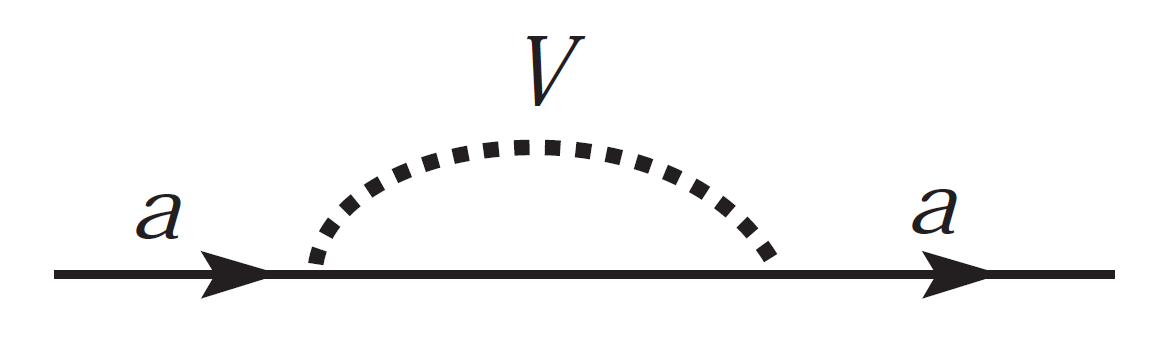
\includegraphics[width=0.6\linewidth]{{C:/Users/Carmen/Desktop/Universidad/TFG/Borradores/img/bettini1.PNG}}
\caption{$V$ emitido y reabsorbido por $a$}
  \label{fig:bettini1}
\end{subfigure}%
\begin{subfigure}{.5\textwidth}
  \centering
  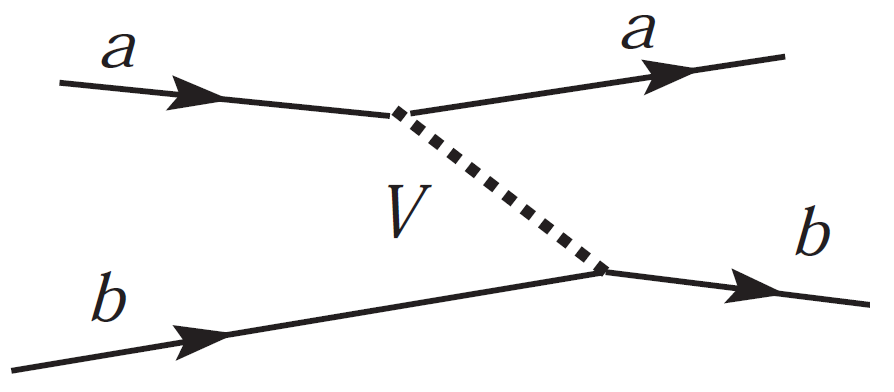
\includegraphics[width=0.6\linewidth]{{C:/Users/Carmen/Desktop/Universidad/TFG/Borradores/img/bettini2.PNG}}
  \caption{$V$ emitido por $a$ y absorbido por $b$}
  \label{fig:bettini2}
\end{subfigure}
\caption[Esquematización del proceso de interacción en TCC]{Proceso de interacción mediante intercambio del bosón mediador.  \cite{Bettini}}
\label{fig:bettini}
\end{figure}

Continuando con el ejemplo anterior, Bettini indica que el bosón mediador $V$ tiene, en general, una masa $m$ no nula, lo que provoca que, durante su emisión, se viole momentáneamente la conservación de energía $\Delta E = m$. Lo mismo, pero de forma opuesta ocurre durante su absorción. Así pues, la violación neta dura un $\Delta t$ y satisface \textit{El Principio de Incertidumbre de Heisenberg}: $\Delta E \Delta t \leq \hbar$, lo que implica que $V$ sólo puede alejarse una distancia finita $R=c\Delta t$. Esta distancia equivale al rango de la fuerza de interacción, por lo tanto, a cuanta mayor masa tenga el bosón mediador de una interacción, menor será su rango de alcance \cite{Bettini}. Dado que los bosones mediadores $W^{\pm}$ y  $Z^0$ tienen masa $m_W$ muy grande, la interacción débil tiene un alcance muy corto, más que cualquier otra interacción fundamental; de ahí la denominación de ``débil''.

Gráficamente, las interacciones se representan con Diagramas de Feynmann. Estos diagramas proporcionan información acerca de la amplitud de probabilidad de los distintos procesos, donde cada línea representa a una partícula y cada vértice corresponde a cada actuación del lagrangiano de la interacción $\mathcal{L}$. Las líneas externas corresponden a partículas reales, mientras que las internas que conectan los vértices representan partículas virtuales, conocidas como propagadores o mediadores. El propagador es la partícula que se crea y aniquila; la que media la interacción. En nuestro ejemplo anterior, dicho propagador sería el bosón $V$  y en el caso de la interacción débil, los propagadores serían los bosones vectoriales $W^{\pm}$ o $Z^0$.







\subsection{Teoría de la Perturbación}\label{sec:perturbation_theory}

\section{Decaimiento de mesones $K$ cargados}
\label{sec:charged_kaon_decay}
\vspace{5mm}